As mentioned in \autoref{sec:design-and-system-architecture}, the software for the system is written in Python and is run entirely on the Raspberry Pi 4B. The software is divided into three main components: the user interface, the computer vision system, and the system controller which manages the hardware components of the system. The software is designed to be modular, with each component being able to run independently of the others. This allows for easier debugging and testing of the system, as well as making it easier to add new features in the future. All written Python code adheres to a style defined in a \texttt{.pylintrc} file, which is a configuration file for the pylint \cite{pylint} linter. This ensures that the code is consistent and readable. The code is also documented using docstrings for readability and maintainability.

All software constants are defined in a \texttt{constants.py} file, which is imported by all other Python files, allowing for easy modification of constants that define the behaviour of the system which is useful for testing and debugging.

Additionally, a lot of thought went into streamlining the development process to ensure that the system is easy to develop and maintain. For example, Visual Studio Code's \cite{vscode} Remote SSH extension is used to develop the system remotely, as it allows developing the system on a much more powerful laptop, while using the familiar VSCode environment with any extensions that help streamline the development process. This is crucial as the Pi is not very powerful, so compiling and running the system on the Pi may be slow and cumbersome.

During development, the Pi connects to the laptop's Wi-Fi hotspot and is configured to be discoverable with the Pi's hostname, facilitating easy access to the Pi through SSH and a VNC Viewer without needing the Pi's IP address, which is dynamic. The Pi also makes use of SSH keys, allowing connection to the Pi without needing to enter a password every time, ensuring quick and easy access.

% Code block
\begin{minipage}[H]{\textwidth}
    \centering
    \begin{minted}[linenos, fontsize=\footnotesize, breaklines, bgcolor=bg]{python}
# Allow development on non-Raspberry Pi devices
try:
    import RPi.GPIO as GPIO # type: ignore
    from rpi_ws281x import PixelStrip, Color
    GPIO.setmode(GPIO.BCM)
    print("Using real hardware!")
except ImportError:
    from src.common.simulate import GPIO
    from src.common.simulate import PixelStrip, Color
    print("Simulating missing hardware!")
    \end{minted}
    \captionof{listing}{Cross-platform GPIO import}
    \label{code:cross-platform-gpio}
\end{minipage}

Additionally, as development is done on both a Windows laptop and the Pi, the code is written to be cross-platform, however certain libraries like the GPIO library are only available on the Pi, so a \texttt{simulate.py} file is used to simulate the GPIO pins on the laptop, allowing for development of the system without needing to be on the Pi as shown in \autoref{code:cross-platform-gpio}.

% Code block
\begin{minipage}[H]{\textwidth}
    \centering
    \begin{minted}[linenos, fontsize=\footnotesize, breaklines, bgcolor=bg]{python}
# Allow development on non-Raspberry Pi devices
class GPIO:
    BCM = 0
    IN, OUT = 0, 0
    HIGH, LOW = 0, 0
    PUD_DOWN, PUD_UP = 0, 0
    FALLING, RISING = 0, 0
    def setmode(_) -> None: pass
    def setup(_, *__, **___) -> None: pass
    def cleanup() -> None: pass
    def output(_, __) -> None: pass
    def add_event_detect(_, *__, **___) -> None: pass
    # PWM emulation
    class PWM:
        def __init__(self, _, __) -> None: pass
        def stop(self) -> None: pass
        def start(self, _) -> None: pass
        def ChangeDutyCycle(self, _) -> None: pass
        def ChangeFrequency(self, _) -> None: pass
    \end{minted}
    \captionof{listing}{Example simulation of the GPIO library}
    \label{code:simulate-gpio}
\end{minipage}

As shown in \autoref{code:simulate-gpio}, the \texttt{simulate.py} file contains a class called \texttt{GPIO} that emulates the GPIO library.

The Pi uses Git \cite{git} for version control, and the repository is hosted on GitHub \cite{github}, with a dedicated branch for the Pi that is regularly updated with the main branch. The vision system and the laptop also maintain their own Git branches which are regularly updated with the main branch, ensuring that all systems are running the same code. This is crucial as it enables development on a more powerful laptop, and then synchronises the changes to the Pi, without having to manually copy any files over. The repository can be found in the Appendix \ref{app:github}.
\subsubsection{User Interface}
The user interface allows the user to view and command the state of the system by interacting with the touchscreen on the DFRobot 7" display. 

Written in pygame \cite{pygamedoc} and pygame\_gui \cite{pygamegui}, the user interface is controlled by the \texttt{LCD UI} class, which is responsible for drawing the various elements of the user interface, such as the camera feed, the buttons, and the text. The system operates at 30Hz, allow for responsiveness without overloading the system. A profiler was used to determine the performance of the system, and it was found that the system was able to run at 30Hz without any issues as discussed in \autoref{sec:electronics-and-software-evaluation}

\begin{figure}[H]
    \hfill
    \begin{minipage}[t]{\textwidth}
      \centering
      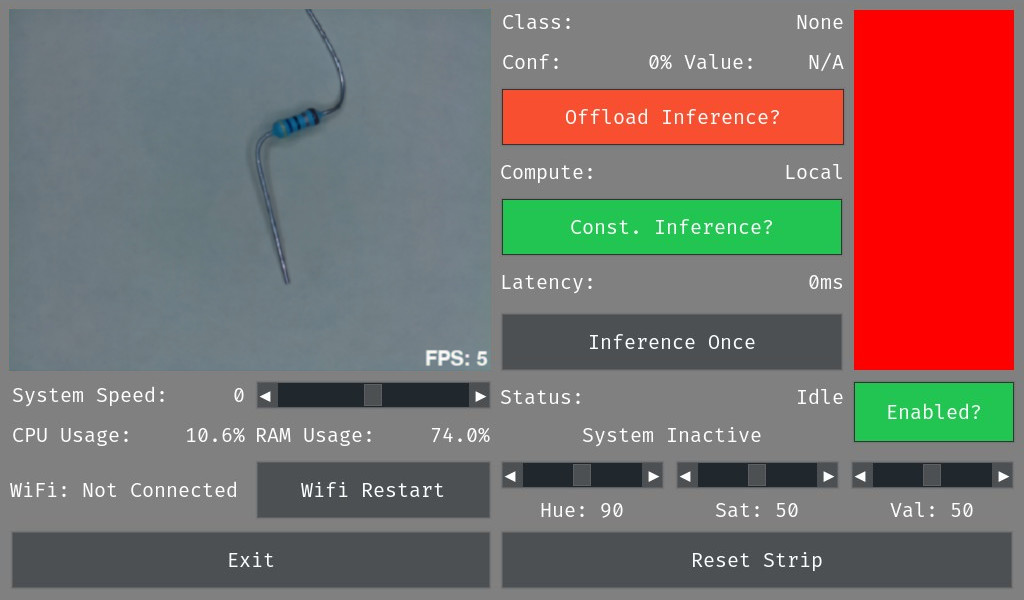
\includegraphics[height=8cm]{imgs/software/screenresistor.jpg}
      \caption{User Interface}
      \label{fig:ui}
    \end{minipage}
\end{figure}

As shown in \autoref{fig:ui}, the user interface consists of a multitude of features that allow the user to interact with the system. The user is able to view the live camera feed, where an inductor is clearly shown on screen. The user is able to adjust the overall system speed by adjusting the slider, which directly affects the System Controller. The CPU and RAM usage of the system is also shown on screen as these can help to judge the load of the system during development, and especially during inference. The colours of important system elements change depending on their value to indicate the state of the system, for example, the CPU and RAM usage are coloured red when they are high, and green when they are low. 

\begin{figure}[H]
    \hfill
    \begin{minipage}[t]{\textwidth}
      \centering
      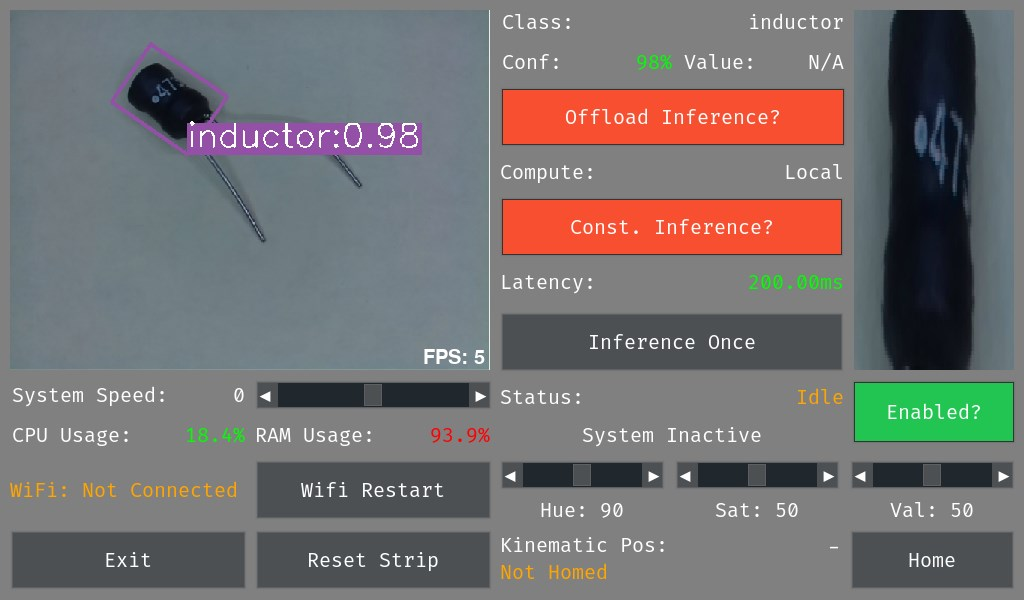
\includegraphics[height=8cm]{imgs/software/screeninference.jpg}
      \caption{Inference Example}
      \label{fig:uiinference}
    \end{minipage}
\end{figure}

On the right side of the screen is information relating to the vision system, for example, what the classification of the component is, its value, and the confidence of the model in its inference. The component is typically displayed in the black area in the top right, as shown in \autoref{fig:uiinference}. As shown in \autoref{fig:uiinference}, the inductor from \autoref{fig:ui} from the live camera feed has been classified as an inductor with a confidence of 98\%. The user interface also shows that inference latency is 200ms. The component is then cropped from its bounding box and then displayed in the top right corner of the screen.

As explained \autoref{sec:software}, the Pi is connected to a more powerful machine with SSH to facilitate faster development. For this reason, a Wi-Fi button is present on the UI to allow it to attempt to reconnect in the event of connection issues. The user interface also supports streaming frames to the machine where inference can be done much quicker, due to the presence of a GPU. This is done by toggling the "Offload Inference?" button. The "Const. Inference?" button means the Vision system is constantly processing frames rather than only when a beam break is detected. The "Inference Once" button allows the user to manually trigger inference, and performs inference on the current frame. 

This was achieved using Python's \texttt{sockets}, \texttt{pickle} and \texttt{multiprocessing} library to facilitate the connection and data transfer between the two devices, and is discussed in more detail in \autoref{sec:concurrency}.

Additionally, during the development of the system, the WS2812B needed to be calibrated as explained in \autoref{sec:ws2812b-led-strip}. Due to this, there are HSV sliders for the user to adjust the colour of the LED strip, allowing for easy calibration of the LED strip. There is also a "Reset Strip" button to reinitialise the LED strip and display the LED start up sequence as shown in \autoref{fig:ledreset}.

The user interface also supports a "training mode" as discussed in \autoref{sec:dataset-collection}, which is done programmatically by toggling a flag called \texttt{TRAININGMODE} in the \texttt{LCD UI} class.
\begin{figure}[H]
    \hfill
    \begin{minipage}[t]{\textwidth}
      \centering
      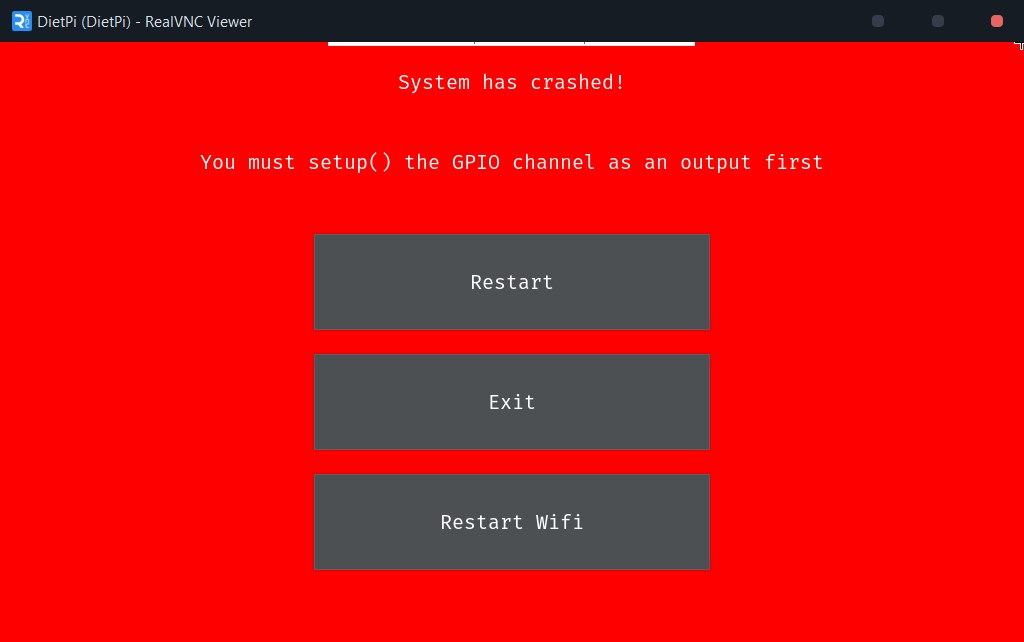
\includegraphics[height=8cm]{imgs/python/systemcrash.jpg}
      \caption{System crash during development}
      \label{fig:crash}
    \end{minipage}
\end{figure}

The LCD UI class is also capable of gracefully handling errors that may occur during the operation of the system, and the handling of these errors is delegated to the specific subsystem that caused the error. If a much more catastrophic error occurs, the system will still gracefully display an error screen, and allow the system to be restarted as shown in \autoref{fig:crash}. This facilitates not only the development process, but also prevents the system from having downtime in real-world applications as it prevents the need for a system restart. This is implemented by making use of Python's exception handling mechanism, and then switching to the error screen if an exception is raised.

The camera feed in the top left is controlled by the Vision Handler, which is responsible for delivering frames to the user interface. The Vision Handler is discussed in more detail in \autoref{sec:vision-handler}. 

\subsubsection{Vision Handler}
\label{sec:vision-handler}
The Vision Handler is responsible for managing the camera feed, and performs the following tasks:
\begin{mylist}
    \item Capturing frames from the camera
    \item Performing inference by passing the frames to the computer vision model
    \item Gracefully handling errors that may occur during inference
    \item Gracefully handling capture errors (such as the camera being disconnected)
    \item The ability to live capture from the \texttt{TRAININGMODE=True} UI mode to allow for development off the Raspberry Pi
\end{mylist}

\autoref{fig:camera-disconnect} shows what the user interface displays when the camera is disconnected.

\begin{figure}[H]
    \hfill
    \begin{minipage}[t]{\textwidth}
      \centering
      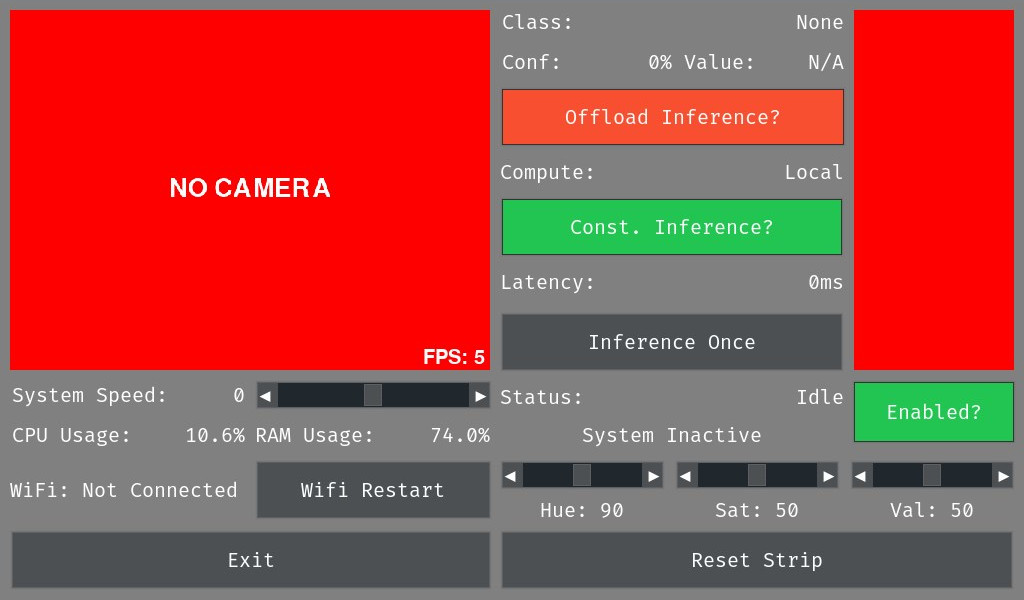
\includegraphics[height=8cm]{imgs/software/screen.jpg}
      \caption{Seamless camera disconnect handling}
      \label{fig:camera-disconnect}
    \end{minipage}
\end{figure}

\subsubsection{System Controller}
\label{sec:system-controller}
The System Controller heavily leverages Python's \texttt{Multiprocessing} library to allow for the system to run multiple processes concurrently, allowing for the system to be more responsive while displaying the \texttt{LCD UI}. The System Controller is responsible for the following tasks:

\begin{mylist}
    \item Detecting a beam break and triggering procedure to sort the component.
    \item Coordinating the movement of the \texttt{Sweeper Controller} to sort the component.
    \item Relaying information back to the \texttt{LCD UI} to display the current state of the system.
    \item Handling the event of the beam break sensor being triggered while the system is in the process of sorting a component.
    \item Handling the event of the endstop being triggered when it is not supposed to be.
\end{mylist}

For the system to reactively sort components, the System Controller uses a beam break sensor to detect when a component is in the sorting area. When the beam break sensor is triggered, the System Controller triggers the \texttt{Sweeper Controller} to sort the component. This is handled using an interrupt, which is a signal that is sent to the CPU to indicate that a system event has occurred, and the CPU should take immediate action. Likewise, the endstop used to detect the sweeper arm's position is also handled using an interrupt to allow it to react in time to prevent damage to the system from the motors. The concurrency of the system is discussed in more detail in \autoref{sec:concurrency}.

\subsubsection{Dataset Collection}
\label{sec:dataset-collection}
As mentioned in \autoref{sec:data-annotation-tool}, a custom dataset annotation tool was used to collect and annotate the dataset required to train the YOLO-OBB model used for component identification, and then extended to train a regular YOLO model for resistor value detection.

\begin{figure}[H]
    \hfill
    \begin{minipage}[t]{\textwidth}
      \centering
      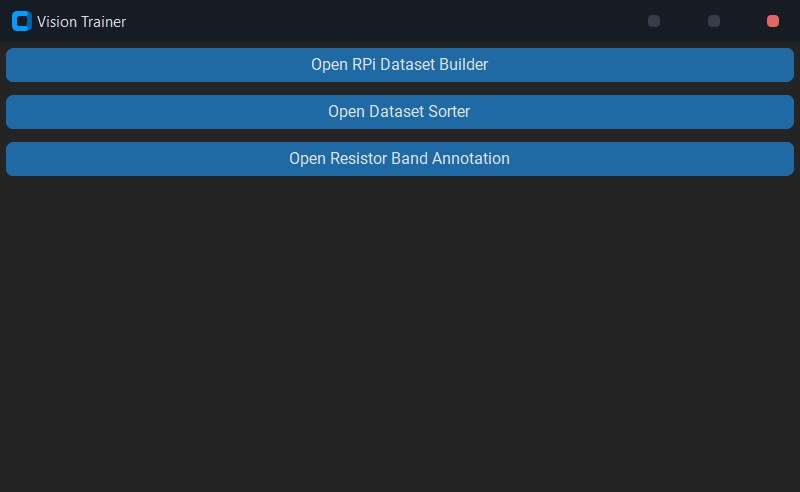
\includegraphics[height=8cm]{imgs/python/visiontrainer.jpg}
      \caption{Vision Trainer Menu}
      \label{fig:vision-trainer}
    \end{minipage}
\end{figure}

Upon launch, the user is able to select which mode they would like to use, as shown in \autoref{fig:vision-trainer}. The user can select the mode by using the following buttons:

\begin{table}[H]
    \centering
    \begin{tabularx}{0.8\textwidth}{|p{3cm}|X|}
        \hline
        \textbf{Button} & \textbf{Action} \\
        \hline
        \oldtexttt{RPi Dataset Builder} & Opens the dataset collection tool, capturing images from the VNC window connected to the Pi \\
        \hline
        \oldtexttt{Open Dataset Sorter} & Opens the dataset sorter tool that sorts a local dataset and reads the labels if they exist \\
        \hline
        \oldtexttt{Open Resistor Band Annotation} & Opens the resistor band annotation tool \\
        \hline
    \end{tabularx}
    \caption{Main buttons for the dataset collection tool}
    \label{tab:dataset-buttons}
\end{table}

\begin{figure}[H]
    \hfill
    \begin{minipage}[t]{\textwidth}
      \centering
      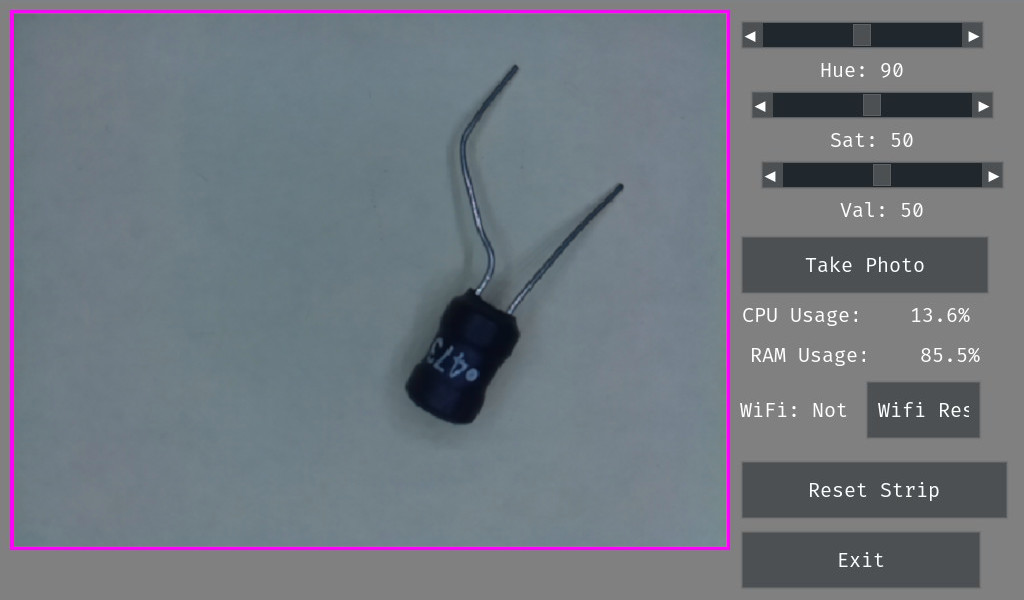
\includegraphics[height=8cm]{imgs/software/trainingmode.jpg}
      \caption{Training Mode Screen}
      \label{fig:training-mode}
    \end{minipage}
\end{figure}

As shown in \autoref{fig:training-mode}, to facilitate the collection of the dataset, the user interface was modified to include a "training mode" that allows the user to capture images of components to be used for training the computer vision system. As the camera feed must originate from the Pi, dataset collection is done on a machine connected to the Pi with VNC \cite{realvnc}, and the user interface is displayed on the VNC client. When \texttt{TRAININGMODE} is enabled, a purple border surrounds the camera feed, enabling the dataset tool to identify where the camera feed is located on the VNC window.

The tool makes use of keybinds to capture images, to allow the user to capture images of components quickly, detailed in the \autoref{tab:keybinds}.

\begin{table}[H]
    \centering
    \begin{tabularx}{0.8\textwidth}{|p{3cm}|X|}
        \hline
        \textbf{Key} & \textbf{Action} \\
        \hline
        \oldtexttt{Space} & Capture from VNC window \\
        \hline
        \oldtexttt{Enter} & Save image but only if the image is captured and labelled \\
        \hline
        \oldtexttt{Escape} & Return to the component selection screen \\
        \hline
        \oldtexttt{Mouse Left Click} & Draw line for OBB \\
        \hline
        \oldtexttt{Mouse Middle Click} & Cancel OBB \\
        \hline
    \end{tabularx}
    \caption{Main keybinds for the dataset collection tool}
    \label{tab:keybinds}
\end{table}

The dataset collection tool uses PyGetWindow \cite{pygetwindow_2020} to identify the VNC window, and PyAutoGUI \cite{pyautogui_2023} to capture the images. OpenCV's \cite{home_2024} \texttt{cv2.findContours} function is used to find the largest contour within the image that is bordered by the purple rectangle, allowing it to effectively extract the camera feed from the VNC window.

% Code block
\begin{minipage}[H]{\textwidth}
    \centering
    \begin{minted}[linenos, fontsize=\footnotesize, breaklines, bgcolor=bg]{python}
    try:
        realVNCWindow = pygetwindow.getWindowsWithTitle(REALVNC_WINDOW_NAME)[0]
        realVNCWindow.activate()
        pygetwindow.getWindowsWithTitle("RPi Dataset Builder")[0].activate()
    except:
        try:
            realVNCWindow = pygetwindow.getWindowsWithTitle("Component Sorter")[0]
            realVNCWindow.activate()
            pygetwindow.getWindowsWithTitle("RPi Dataset Builder")[0].activate()
        except:
            self.imgBorder.configure(bg_color=BORDER_COLOUR_FAILED)
            print("No Window Found")
            return
    # Capture the image
    screenshotPil = pyautogui.screenshot(region=(realVNCWindow.left, realVNCWindow.top, realVNCWindow.width, realVNCWindow.height))
    # Convert to OpenCV format
    screenshotCv = numpy.array(screenshotPil)
    # Find the contours defined by the pink square
    mask = cv2.inRange(cv2.cvtColor(screenshotCv, cv2.COLOR_BGR2HSV), LOWER_THRESHOLD, UPPER_THRESHOLD)
    contours, _ = cv2.findContours(mask, cv2.RETR_TREE, cv2.CHAIN_APPROX_SIMPLE)
    \end{minted}
    \captionof{listing}{Camera feed extraction from VNC window}
\end{minipage}

\begin{figure}[H]
    \hfill
    \begin{minipage}[t]{\textwidth}
      \centering
      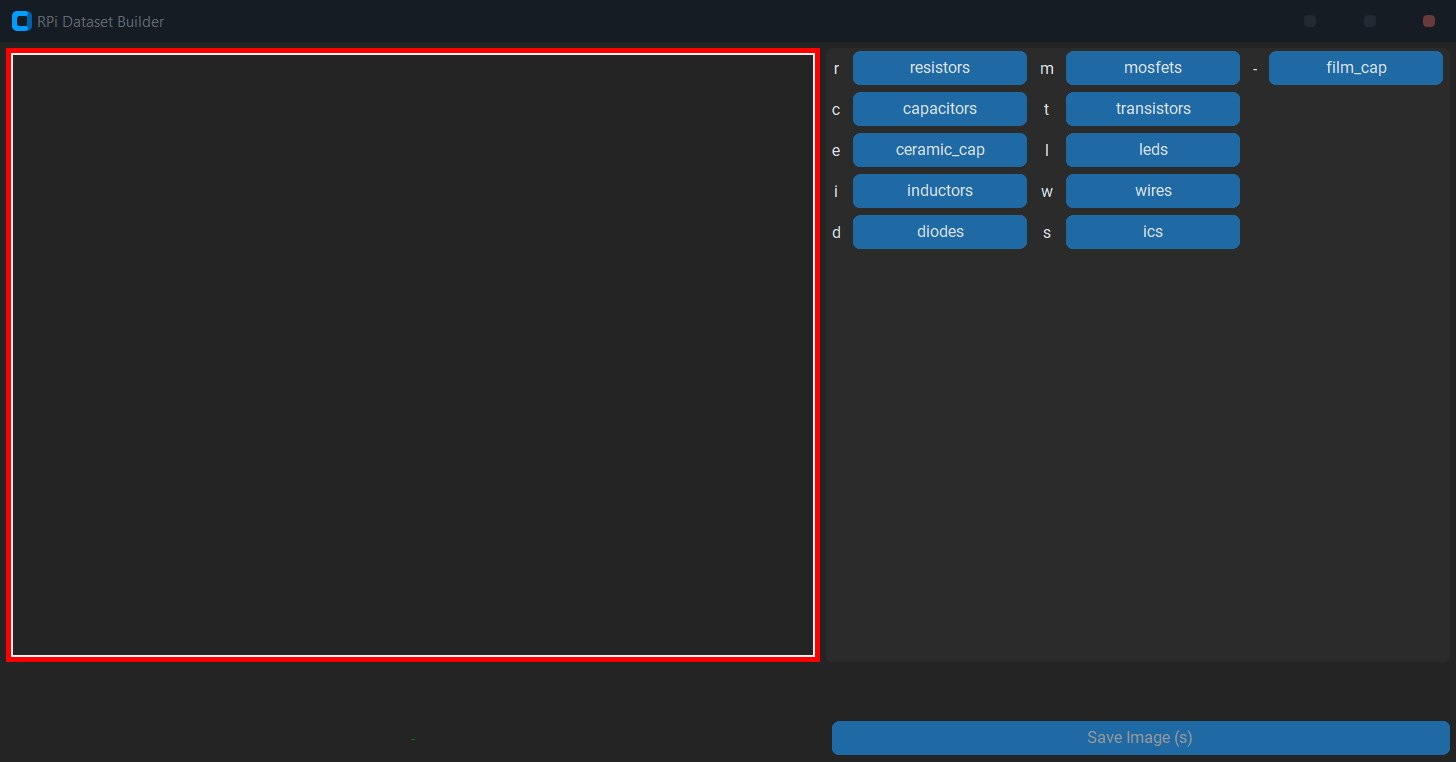
\includegraphics[height=8cm]{imgs/python/uncaptured.jpg}
      \caption{Uncaptured camera feed with red border}
        \label{fig:uncaptured}
    \end{minipage}
\end{figure}

If the camera feed is not captured (it may be obscured), the border of the camera feed will turn red, as shown in \autoref{fig:uncaptured}, indicating that the camera feed was not captured, otherwise it will turn green, as shown in \autoref{fig:captured}. In \autoref{fig:uncaptured}, the user is selecting which component to sort on the component selection screen, and has a selection from the following components: 
\begin{multicols}{2}
    \begin{mylist}
        \item Resistors
        \item Capacitors
        \item Ceramic Capacitors
        \item Inductors
        \item Diodes
        \item MOSFETs
        \item Transistors
        \item LEDs
        \item Wires
        \item ICs
        \item Film Capacitors
    \end{mylist}
\end{multicols}

The user can select the component to sort by clicking on the component button or by using the hotkey indicated to the left of the button.  

\begin{figure}[H]
    \hfill
    \begin{minipage}[t]{\textwidth}
      \centering
      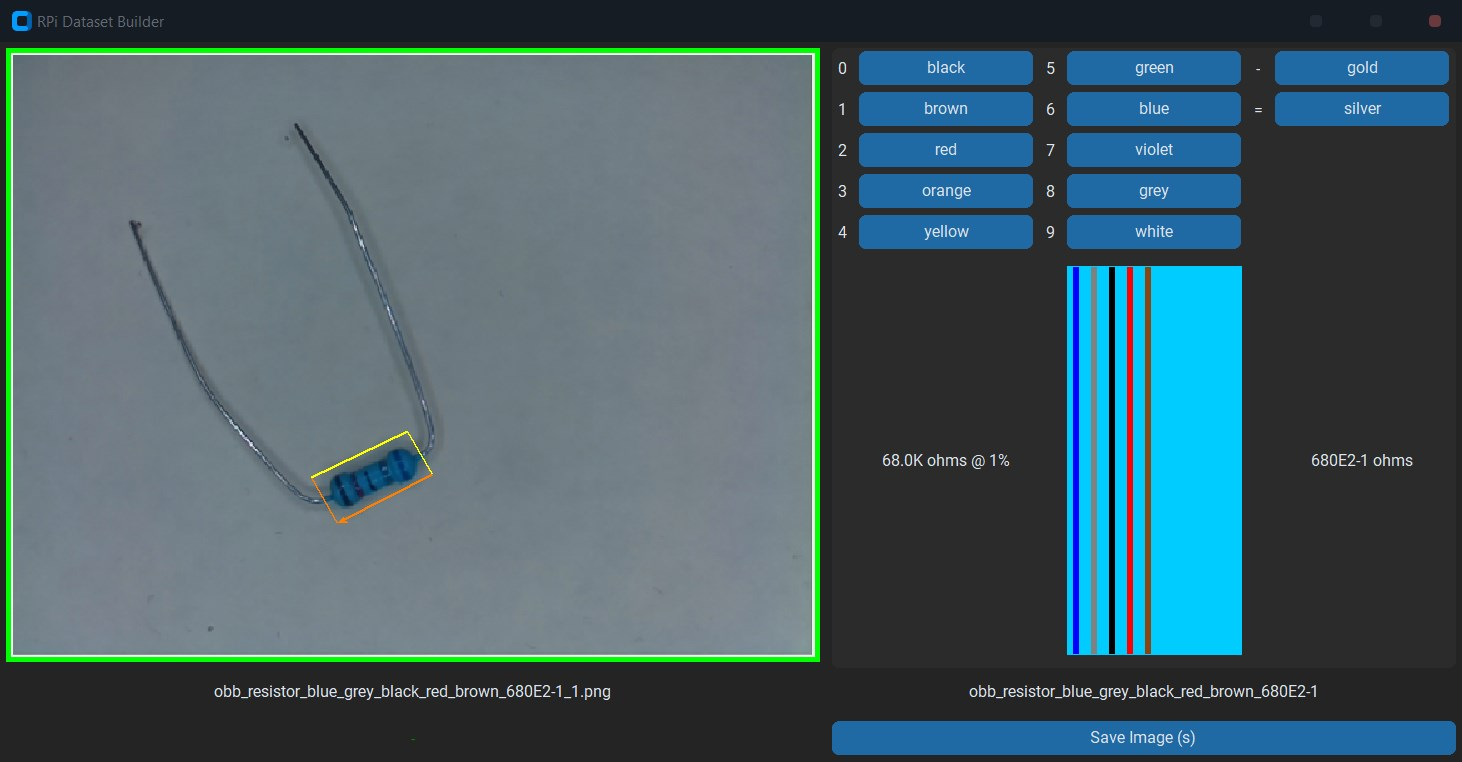
\includegraphics[height=8cm]{imgs/python/captured.jpg}
      \caption{Successfully captured camera feed with green border and annotated resistor}
        \label{fig:captured}
    \end{minipage}
\end{figure}

In \autoref{fig:captured}, the user has successfully captured the camera feed, and has annotated a resistor. The tool has hotkeys for quickly annotating the band and retains the configuration of the band between images, allowing for quick annotation of resistors (as the user would take multiple angles of the same resistor). During band annotation, the program automatically calculates what the value of the resistor should be, including tolerances, and displays this on the screen, to help prevent the mislabelling of the resistors. The bands and value are then saved in the filename of the image and label, allowing the resistor value model to be trained based off the file names. For eaxmple, in \autoref{fig:captured}, the resistor will be saved as \texttt{obb\_resistor\_blue\_grey\_black\_red\_brown\_680E2-1\_1.png}; the value of the resistor is 68 k$\Omega$, with a tolerance of 1\% and is the first image of this value in the dataset.

The user can also draw the OBB by clicking and dragging the mouse, and can cancel the OBB by clicking the middle mouse button. The tool automatically connects the first and last points to form the OBB, showing a gray dotted line so the user can verify the OBB is correct. The user can then save the image by pressing the \texttt{Enter} key, or return to the component selection screen by pressing the \texttt{Escape} key.

Originally, it was thought that the OBB model learns the correct left-right orientation of objects by the order of which the vertexes are joined, and this is represented in the tool with two orange arrows, showing the desired right-side up orientation of the resistor. However, this was found to be incorrect, and the OBB model only learns the bounding box of the object, and not the orientation of the object. This was discovered during the training of the OBB model, as discussed in \autoref{sec:computer-vision}

\begin{figure}[H]
    \hfill
    \begin{minipage}[t]{0.45\textwidth}
      \centering
      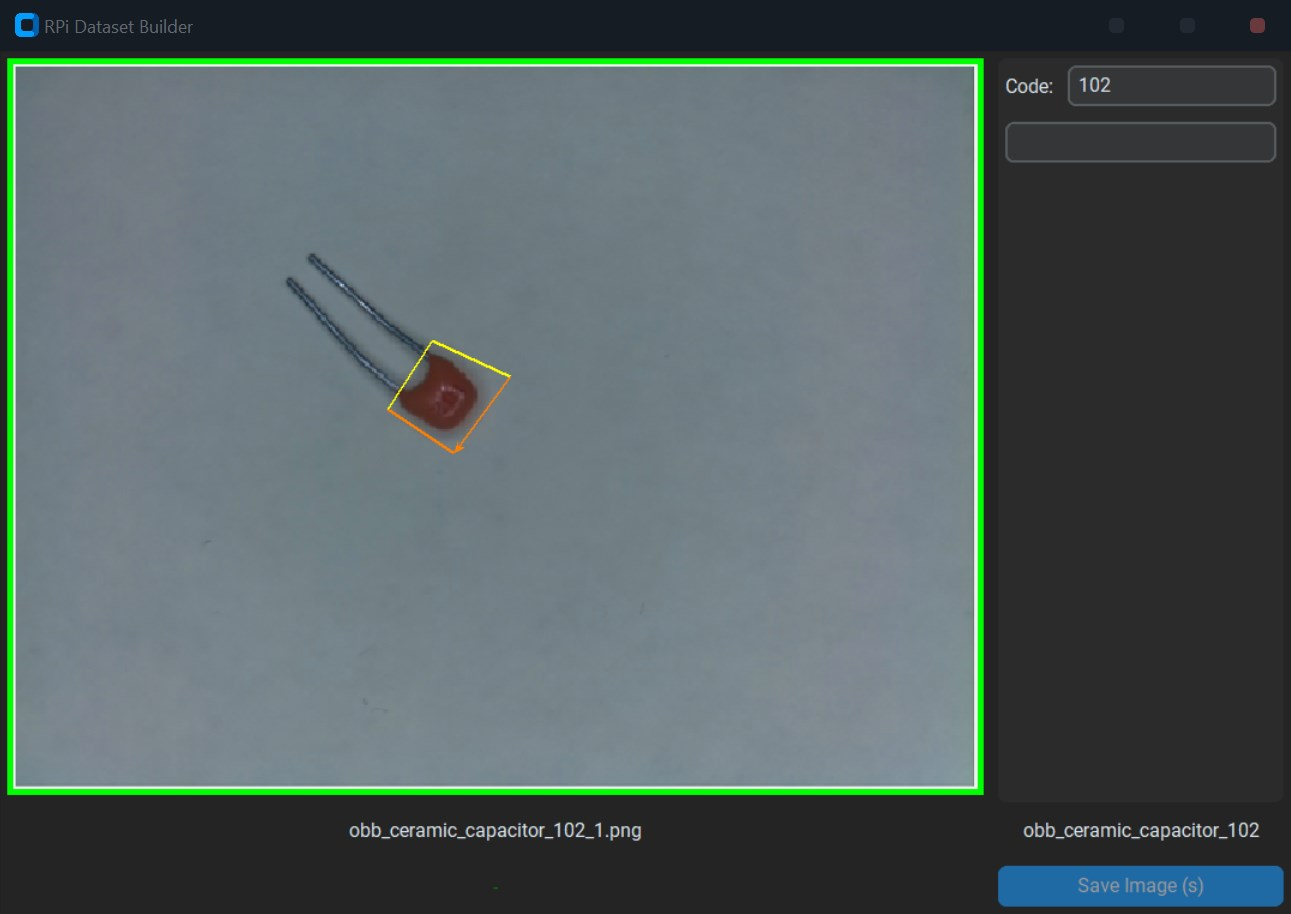
\includegraphics[width=\columnwidth]{imgs/python/capcapture.jpg}
      \caption{Annotated Ceramic Capacitor}
      \label{fig:capcapture}
    \end{minipage}
    \hfill
    \begin{minipage}[t]{0.45\textwidth}
      \centering
      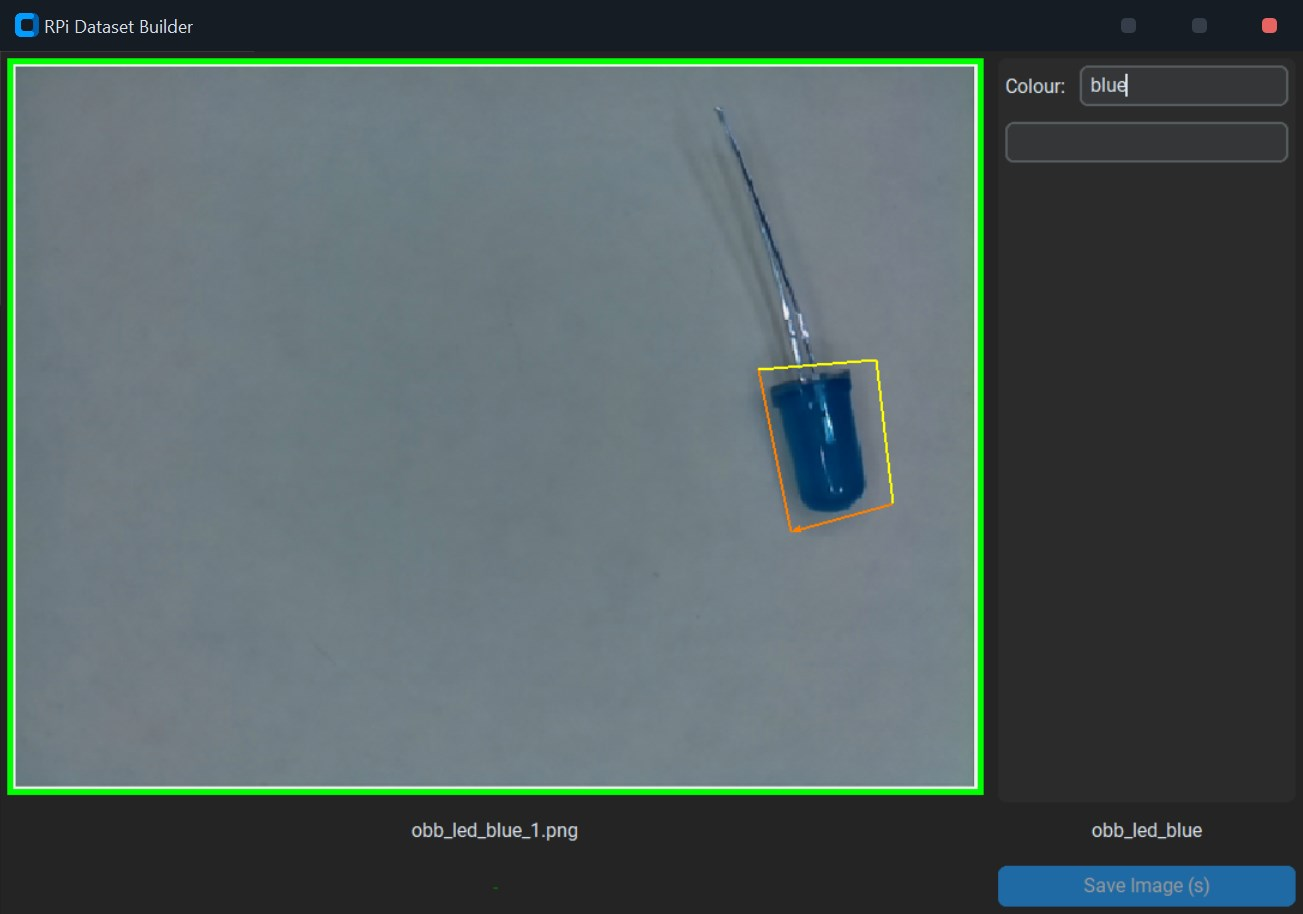
\includegraphics[width=\columnwidth]{imgs/python/ledcapture.jpg}
      \caption{Annotated LED}
      \label{fig:indcapture}
    \end{minipage}
    \hfill
\end{figure}

\autoref{fig:capcapture} shows an annotated ceramic capacitor, and \autoref{fig:indcapture} shows an annotated LED, demonstrating the tool's ability to annotate components of different shapes and sizes.

In addition to regular component identification using the YOLO-OBB model, a separate model was trained to identify the value of resistors, which is discussed in more detail in \autoref{sec:computer-vision}. This dataset is collected by using the classification model to identify the resistor, and then the bounding box is used to crop the image to the resistor. The cropped image then contains the neccessary information to train the resistor value model, such as the bands and the value of the resistor, but is missing the location of the bands in the image, and the orientation of the resistor, which would help it determine what the first band is. This means a tool is still required to annotate the resistor bands.

\begin{figure}[H]
    \hfill
    \begin{minipage}[t]{\textwidth}
      \centering
      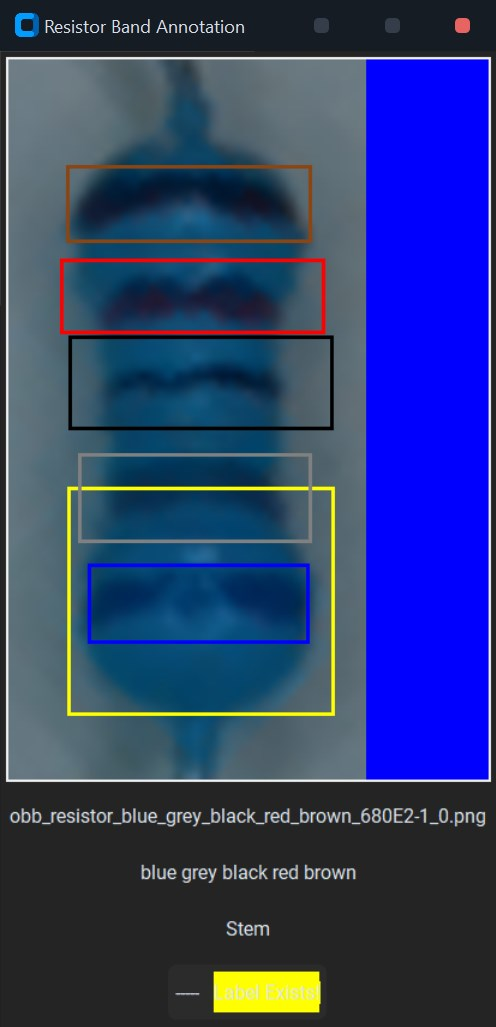
\includegraphics[height=8cm]{imgs/python/resistorannotate.jpg}
        \caption{Resistor band annotation tool}
        \label{fig:resistorannotate}
    \end{minipage}
\end{figure}

As shown in \autoref{fig:resistorannotate}, the tool clearly shows a resistor being annotated, with the bands being drawn on the resistor. The user only has to click on the location of the bands, and does not need to manually annotate what band the user is clicking on; the information of the order of the bands in encoded in the filename as discussed earlier, so the tool can automatically determine what band the user is clicking on. The user only needs to indicate where the 'stem' of the resistor is, indicated by the yellow box, enabling the tool to identify the orientation of the resistor, and then allowing the resistor value model to be trained. Clicking on the resistor automatically draws a bounding box centered at the band location with the current band colour, and then saves the image and label in the same way in the YOLO format (not the YOLO-OBB format as the component identification model will always produce resistors upright). The format is discussed in more detail in \autoref{sec:computer-vision}. 

\subsubsection{Concurrency and Optimisation}
\label{sec:concurrency}
To ensure that the system is responsive and can handle multiple tasks concurrently, the system makes use of Python's \texttt{multiprocessing} library to run multiple processes concurrently. The system is divided into three main processes: the main process, the vision process, and the system controller process.

The main process is responsible for running the user interface, and it has the highest priority as it is responsible for displaying the state of the system to the user and must be responsive to user input. This is achieved by using an event loop to handle user input, and then updating the user interface accordingly, and also ensuring that no blocking operations are performed in the main process. A blocking process is an operation that pauses the execution of code until it is complete, and would prevent the event loop from executing and would "freeze" the user interface. To prevent this, all blocking operations are delegated to other processes, and the main process only waits for the results of these operations.

Pygame and Pygamegui make event handling easy, as they provide an event queue that allows the system to consume events as they occur, and then update the user interface accordingly. This allows the system to be responsive and handle multiple tasks concurrently. 

The vision process is responsible for capturing frames from the camera, and then passing these frames to the computer vision model for inference. Inference must be run on a separate process due to the fact that inference is computationally expensive, making it a blocking operation as the system must wait for the inference to complete before it can continue. This has been achieved by using Python's \texttt{multiprocessing} library to run the vision process concurrently with the main process, allowing the system to capture frames and perform inference at the same time.

% Code block
\begin{minipage}[H]{\textwidth}
    \centering
    \begin{minipage}[H]{\textwidth}
    \centering
    \begin{minted}[linenos, fontsize=\scriptsize, breaklines, bgcolor=bg]{python}
model = YOLO(modelPath)
print("Loaded YOLO model!")
while True:
    print("Waiting for frame")
    frame = frameQueue.get()
    start = time.time()
    print("Got frame")
    # Inference
    prediction = model.predict(frame)
    results = draw_results(frame, prediction)
    resultQueue.put(results)
    busyInference.clear()
    print(f"Inference took {time.time()-start:.2f}s")
    \end{minted}
\end{minipage}
\begin{minipage}[H]{\textwidth}
    \centering
\begin{minted}[linenos, fontsize=\scriptsize, breaklines, bgcolor=bg]{python}
# Consume the result
if not self.resultQueue.empty():
    results = self.resultQueue.get()
    endTime = time.time()
    # Update the LCD
    ...
# Produce a frame
if (self.doInference.is_set() or self.constInference.is_set()) and not self.busyInference.is_set():
    self.busyInference.set()
    if self.frameQueue.empty():
        self.startTime = time.time()
        self.frameQueue.put(pygame.surfarray.array3d(frame).swapaxes(0,1))
        self.doInference.clear()
        \end{minted}
    \captionof{listing}{Producer and Consumer mechanism for the Vision Handler}
    \label{code:producer-consumer}
    \end{minipage}
\end{minipage}

In \autoref{code:producer-consumer}, the vision process is shown to be a producer-consumer mechanism, where the inference process (top) is the producer, and the main process (bottom) is the consumer. The mechanism makes use of multiprocessing queues and events which are multiprocessing synchronisation primitives that allow for the communication between processes without the need for locks to ensure data integrity. If the same data is accessed by multiple processes at the same time, it can lead to data corruption, or race conditions, which can cause the system to behave unpredictably. The queues and events ensure that the data is accessed in a multiprocessing-safe manner, and that the processes are able to communicate effectively.

In this mechanism, the main process ensures that the frame queue is empty before putting a frame into the queue, and then sets the \texttt{doInference} event, which signals to the vision process that a frame is ready for inference. This check is necessary as the "put" operation is blocking, and will wait until the queue is empty before putting the frame into the queue, as its maximum length was set to 1. The vision process then waits for the \texttt{doInference} event to be set, and then performs inference on the frame, and then puts the result into the result queue. The main process then consumes the result from the result queue, checking if the result queue is empty for the same reason, before consuming the result. This mechanism successfully allows the vision process to perform inference concurrently with the main process, and ensures that the system is responsive and can handle multiple tasks concurrently.

Note that Python's \texttt{threading} library cannot be used for this purpose, as Python's Global Interpreter Lock (GIL) prevents multiple threads from executing Python code concurrently, and only allows one thread to execute Python code at a time. This makes it useful for I/O-bound tasks, but not for CPU-bound tasks, as the GIL would prevent the inference from taking place while the main process is running.

For offloaded inference to a more powerful machine, the system uses Python's \texttt{sockets} library to establish a connection between the Pi and the machine, and then uses Python's \texttt{pickle} library to serialise the frame and send it over the network. As the Pi is connected to the machine via its own Wi-Fi hotspot, a connection is easily established and frames can be sent over the network. The machine then deserialises the frame, performs inference, and then sends the results back to the Pi, which then displays the results on the user interface. This operation is I/O-bound, and could be threaded using Python's \texttt{threading} library, but as the system is already using \texttt{multiprocessing} and supports toggling between offloaded and on-device inference, it was decided to keep using \texttt{multiprocessing} for development simplicity.

For the system controller, the system controller process is responsible for detecting a beam break, and then triggering the system to sort the component. The beam-break is detected by the system controller using an interrupt using Python's \texttt{RPi.GPIO}, and then the system controller triggers a process to begin sorting the component.

Additionally, to ensure that the system has all the computational resources it needs to run effectively, the system runs off a minimal environment, with no desktop environment. To display the user interface, the system uses a custom "startx" session that only starts the necessary processes, and reduces the overhead of running a full desktop environment. "startx" is a program that starts the X Window System server and the X Window System, allowing GUI applications to be run on the system. Pygame has the capability to display to a minimal X server, and this helped to influence the design choice of picking Pygame as the user interface library.


